\part{Step Counter Algorithm}

    \chapter{Overview}

        This section covers the development and evaluation of the step counter algorithm. The algorithm aims to extract incidences of steps from the raw accelerometer data recorded on a smartphone. An example of raw accelerometer data of walking is shown below in Figure \ref{img_accel_ex}. It should be quite clear that the act of walking gives rise to periodic activity with a period corresponding to a single step. The act of walking is detailed in Naqvi, et. al. [CIT] and is as follows:

        \begin{enumerate}
            \item At the beginning of the step, the planted foot is pushed backwards into the floor.
            \item Static friction opposes this force. This provides the driving force forward.
            \item At the end of the step the stepping foot is placed on the floor and pushes forward into the floor.
            \item Again, static friction opposes this force, giving rise to a backwards force.
        \end{enumerate}

        \begin{figure}[h]
            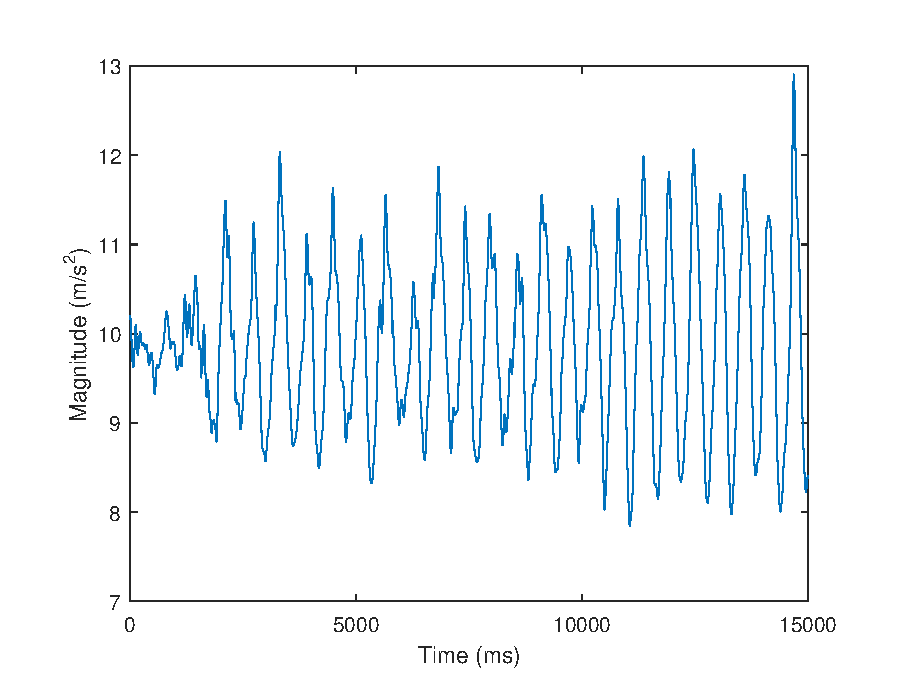
\includegraphics[width=\textwidth]{Images/accel_signal.eps}
            \centering
            \caption{Example of an accelerometer signal recorded during a period of walking.}
            \label{img_accel_ex}
        \end{figure}

        It is clear that each step will have both a peak and a trough associated with 2 and 4 respectively. The algorithm shall identify the peaks in the accelerometer signal. Effectively, the problem is one of peak detection in a noisy signal. 

        The algorithm is split into five stages, each responsible for a particular function. The data flows from stage to stage. All stages have an input data stream and output data stream, with the exception of the final stage which only has an input data stream. A block diagram is shown below in Figure \ref{img_sc_block}. Each one of the five stages will be described in detail in the following section. Note that throughout the description there will be options or parameters for each stage; this is intentional, as this allows an optimization routine to be ran on the algorithm to determine the best set of parameters for overall accuracy. 

        \begin{figure}[h]
            \includegraphics[width=\textwidth]{Images/step_counter_block.png}
            \centering
            \caption{Block diagram of the step counter algorithm.}
            \label{img_sc_block}
        \end{figure}

    \chapter{Algorithm Description}

        \section{Pre-Processing Stage}

            The Pre-Processing Stage is responsible for two functions:

            \begin{enumerate}
                \item Formatting the data received from the accelerometer into a usable format.
                \item Ensuring a constant sampling frequency by means of linear interpolation.
            \end{enumerate}

            The accelerometer data is received in the tri-axial format, however the algorithm is concerned with the magnitude rather than any single directional component because the the physical orientation of the device is unknown. The time stamps of the samples should also be scaled appropriately so that the first sample received from the user initiating the algorithm is at $t = 0$. The time stamps of the samples are provided in nanoseconds and are not given in standard UTC format, but as the time since system boot. The equations for these operations are simple and are as follows:

            \begin{equation}
                m = \sqrt{a_{x}^2 + a_{y}^2 + a_{z}^2},
            \end{equation}

            \begin{equation}
                t_{i,adjusted} = \frac{t_i - t_0}{t_s},
            \end{equation}

            where $m$ is the magnitude of the acceleration signal, $a_{x}$ is the acceleration in the x direction, $a_{y}$ is the acceleration in the y direction, $a_{z}$ is the acceleration in the z direction, $t_{i,adjusted}$ is the adjusted time stamp for the i-th sample, $t_i$ is the time stamp for the i-th sample, $t_0$ is the first time stamp in the trace, and $t_s$ is the time-scaling factor. For example, converting from nanoseconds to milliseconds, $t_s = 10^6$. 

            The data is then inserted into a simple data structure and is appended to an internal buffer of size 2. When this buffer is full, we will interpolate between these two points. The reason interpolation is needed is that although the developer can specific a desired sample rate in the Android application, there is no guarantee that the accelerometer will be sampled at this rate. An example of this is shown below in Figure \ref{img_sampling_freq} where time between samples is plotted against samples. For the filtering stage, we need to ensure that the data is sampled at a constant rate.

            The algorithm knows what the desired sample rate is, and will interpolate at this value. For example, if the sample rate is set to $f = 100 Hz$, then the algorithm will interpolate around $t = 0, 10, 20, 30, ... ms$. Each interpolated point is appended to the end of the stage's output data stream. The pseudocode for the linear interpolation is shown below.

            The equation for linear interpolation is as follows:

            \begin{equation}
                value = \frac{y_1 - y_0}{t_1 - t_0} t_{int} + y_0,
            \end{equation}

            where the two points that are being interpolated between are given by: $(t_1, y_1)$ and $(t_0, y_0)$, and the time to be interpolated at is given by $t_{int}$.

            \begin{figure}[h]
                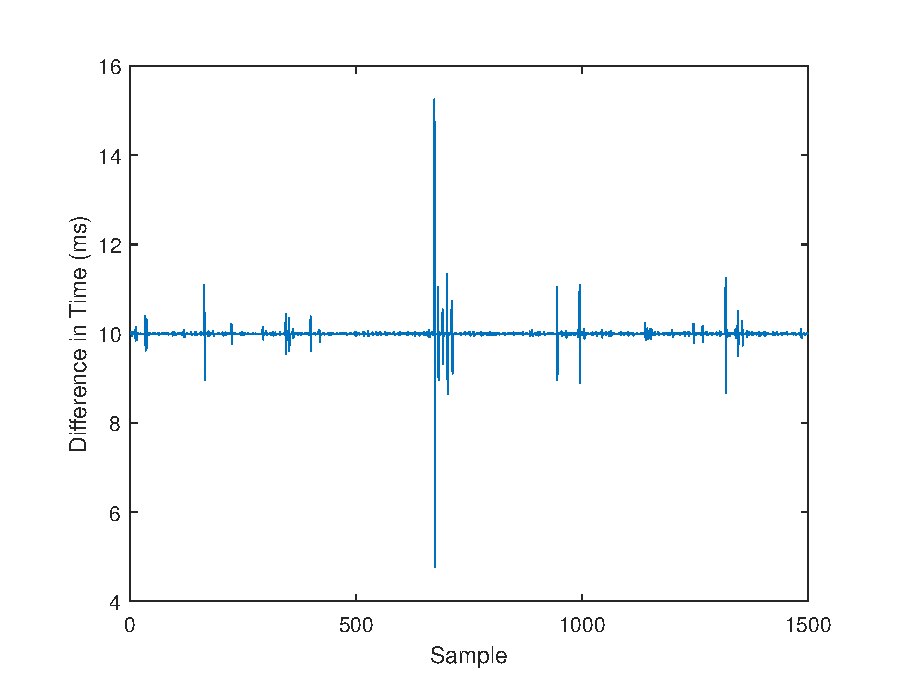
\includegraphics[width=\textwidth]{Images/sampling_freq.eps}
                \centering
                \caption{Time differences between samples for a 100Hz sampled signal. Note that the non-constant sampling times leads to the requirement for interpolation.}
                \label{img_sampling_freq}
            \end{figure}

        \section{Filtering Stage}

            The function of the filtering stage is to smooth the signal by removing as much of the high frequency noise from the acceleromater as possible.

            The filter required is a simple finite impulse response (FIR), low-pass digital filter. Ideally, this would be a steep-low pass filter with a frequency response described by Figure \ref{img_ideal_filter} below. However, this is impossible to achieve due to the infinite impulse response in the time domain (top-hat transforms to the sinc function). In order to capture the a variety of walking speeds, the cutoff of these filters will aim to be around 3 Hz. This should be sufficient to capture the walking of even the speediest walkers, as this would translate to an pace of $5.4 mph$ according to the ratio of $2000 steps = 1 mile$ as given by the American College of Sports Medicine [CIT]. Note that the average walking pace was found to be $3.1 mph$ in a study by Knoblauch, et. al. [CIT].

            An example of the prefiltered signal and the filtered signal is shown below in Figure \ref{img_filtered_signal}.

            \begin{figure}[h]
                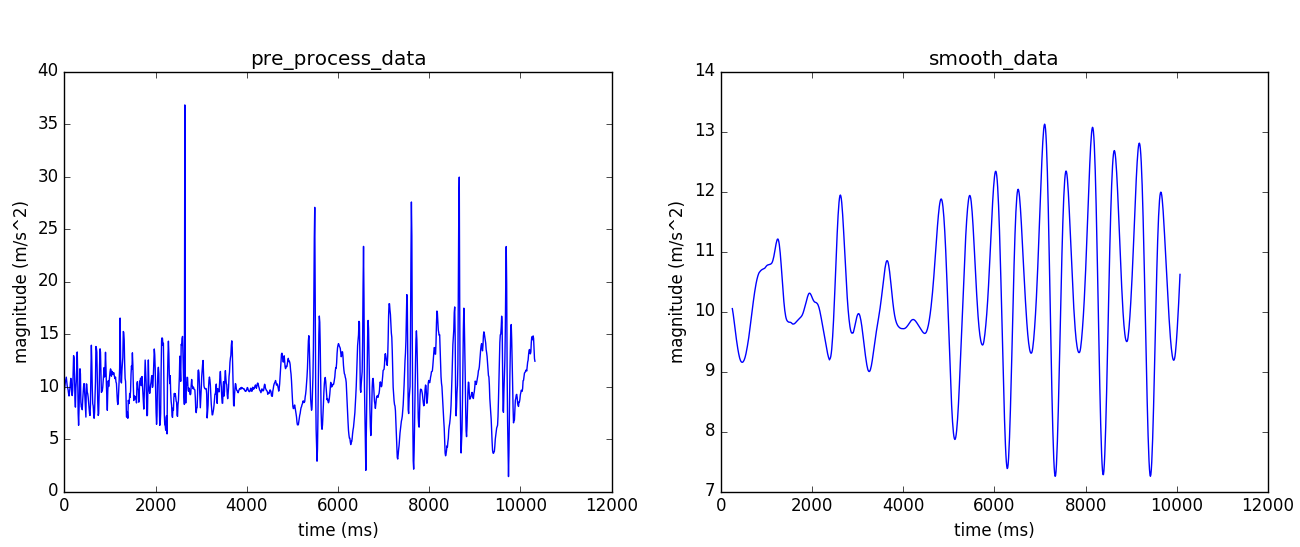
\includegraphics[width=\textwidth]{Images/filtered_signal.png}
                \centering
                \caption{Example of a signal being filtered. Filter used: Gaussian Filter with $N=51$ and $\sigma=0.35$. Note the large peaks due to noise are filtered out entirely.}
                \label{img_filtered_signal}
            \end{figure}

            A few filters were implemented for performance testing.

            \subsection{Moving Average}

                This is a very simple filter, each point in the filter window are weighted equally such that:

                \begin{equation}
                    m_k = \frac{1}{N},
                \end{equation}

                where $m_k$ is the $k^{th}$ filter coefficient, and $N$ is the length of the filter. The frequency response of this filter is shown below in Figure \ref{img_cm_filter}.

                \begin{figure}[!th]
                    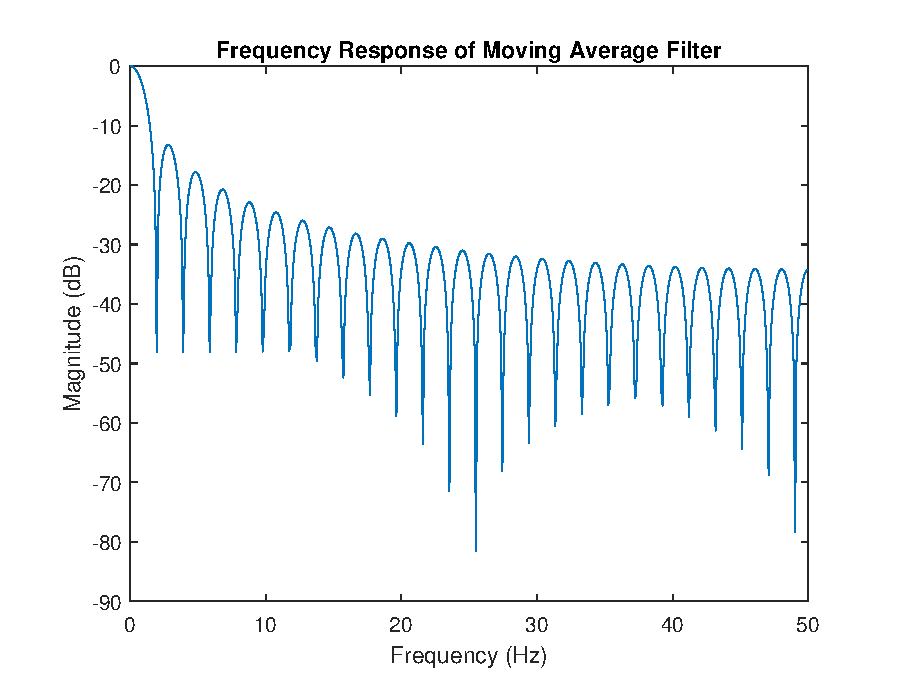
\includegraphics[width=\textwidth]{Images/cm_filter.eps}
                    \centering
                    \caption{Frequency response of the moving average filter with $N=31$.}
                    \label{img_cm_filter}
                \end{figure}

            \subsection{Gaussian Filter}

                This is a more complex filter, using a Gaussian as the waveform for the filter coefficients. This filter attempts to suppress the sidelobes of the center moving average filter by having a smoother transition to 0 magnitude. The weights of the filter are given by:

                \begin{equation}
                    g_k = \exp(-\frac{1}{2}(\frac{k - \frac{N-1}{2}}{\sigma \frac{N-1}{2}})^2),
                \end{equation}

                where $g_k$ is the $k^{th}$ coefficient of the filter, $N$ is the length of the filter window, and $\sigma$ is a parameter defining the standard deviation of the Gaussian. Note that the standard deviation also scales with the length of the filter. The frequency response of this filter is shown below in Figure \ref{img_ga_filter}.

                \begin{figure}[!th]
                    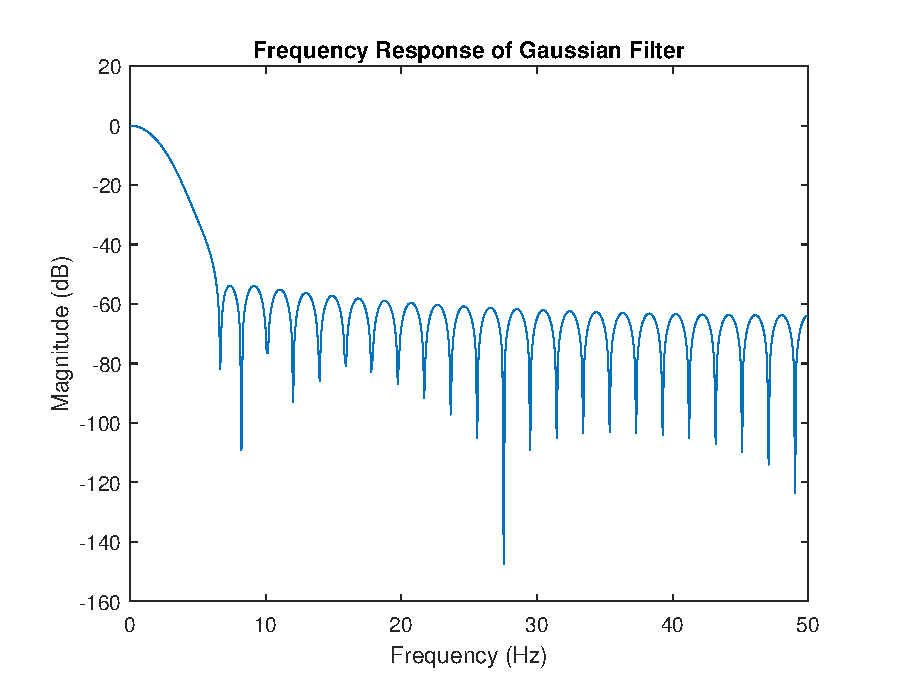
\includegraphics[width=\textwidth]{Images/ga_filter.eps}
                    \centering
                    \caption{Frequency response of the Gaussian filter with $N=51$ and $\sigma = 0.35$.}
                    \label{img_ga_filter}
                \end{figure}

            \subsection{Hann Filter}

                This is a similar filter to that of the Gaussian, where it attempts to smooth out the response by suppressing the sidelobes of the center moving average filter. The weights of the filter are derived from the Hann window [CIT] and are as follows: 

                \begin{equation}
                    h_k = \frac{1}{2}(1 - \cos(\frac{2\pi k}{N - 1}))
                \end{equation}

                where $h_k$ is the $k^{th}$ filter coefficient and $N$ is the length of the filter window. The frequency response of this filter is shown below in Figure \ref{img_ha_filter}.

                \begin{figure}[!th]
                    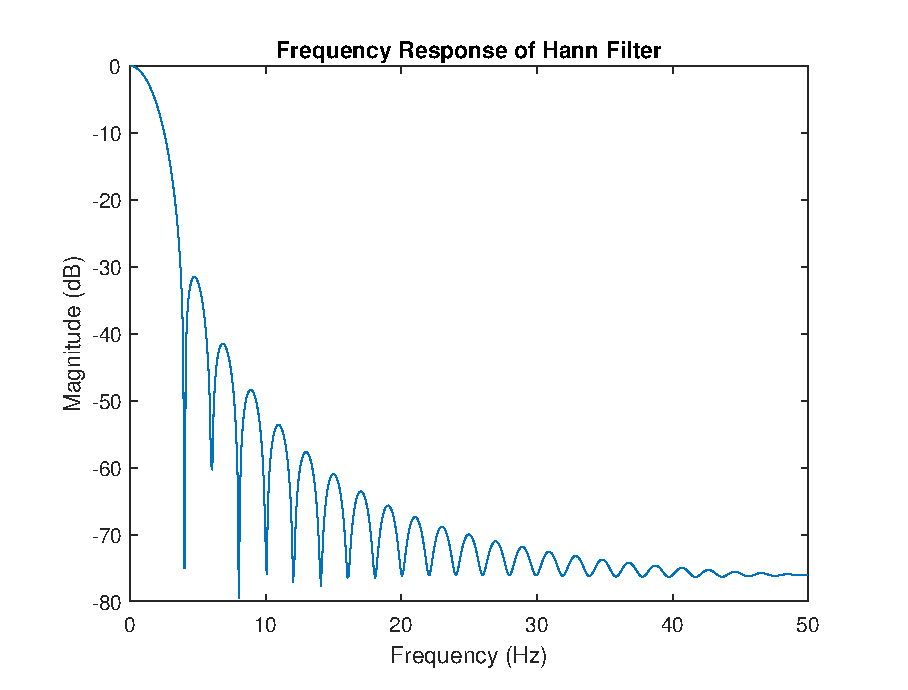
\includegraphics[width=\textwidth]{Images/ha_filter.eps}
                    \centering
                    \caption{Frequency response of the Hann filter with $N=51$.}
                    \label{img_ha_filter}
                \end{figure}  

            \subsection{Kaiser-Bessel Filter}

                This is the most complex filter design, designed by Kaiser [CIT] in order to achieve the desired attenutation at the cutoff frequency. It combines the ideal filter response (note a sinc function in the time domain) and a Bessel window to achieve the result. The calculation of the coeffcients are as follows.

                First, calculate the window shape parameter $\alpha$. 

                \begin{equation}
                    \alpha = 
                        \begin{cases}
                            0.1102(A - 8.7) & A \ge 50 \\
                            0.5842(A-21)^{0.4} + 0.07886(A-21) & 21 \leq A \geq 50 \\
                            0 & A \le 21
                        \end{cases},
                \end{equation}

                where $A$ is the desired attenuation at the cutoff frequency.

                Then calculate the coefficients of the Kaiser-Bessel window:

                \begin{equation}
                w_k = \frac{I_0(\alpha \sqrt{1 - (\frac{k - N_p}{N_p})^2})}{I_0(\alpha)},
                \end{equation}

                where $w_k$ is the $k^{th}$ coefficient of the window, $\alpha$ is the window shape parameter, $N_p$ is the midpoint of the filter, $N_p = \frac{N-1}{2}$ where $N$ is the length of the filter, and $I_0$ is the $0^{th}$ order Bessel function of the first kind.

                Then calculate the coefficients of the ideal filter response:

                \begin{equation}
                i_k = \frac{\sin(2\pi k\frac{F_c}{F_s})}{\pi k},
                \end{equation}

                where $i_k$ is the $k^{th}$ coefficient of the ideal filter response, $F_c$ is the desired cutoff frequency and $F_s$ is the sampling frequency.

                Finally, compute the coefficients of the filter with: 

                \begin{equation}
                b_k = w_ki_k,
                \end{equation}

                where $b_k$ is the $k^{th}$ coefficient of the Kaiser-Bessel filter response. The frequency response of this filter is shown below in Figure \ref{img_kb_filter}.

                \begin{figure}[!th]
                    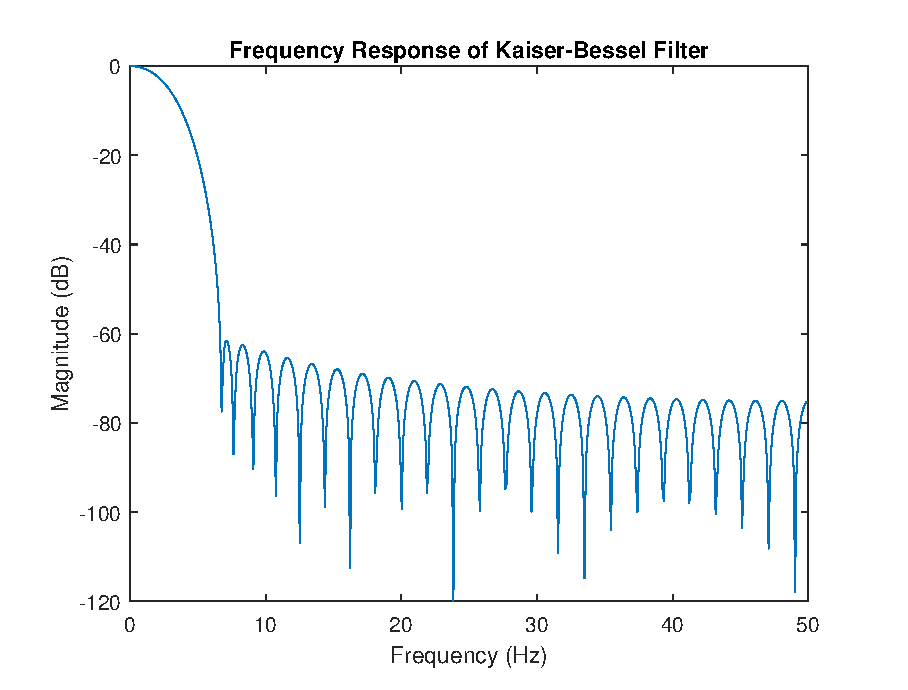
\includegraphics[width=\textwidth]{Images/kb_filter.eps}
                    \centering
                    \caption{Frequency response of the Kaiser-Bessel filter with $N=51$, $A=60dB$, $F_c = 3Hz$, and $F_s= 100Hz$.}
                    \label{img_kb_filter}
                \end{figure}  

        \section{Scoring Stage}

            The function of the scoring stage is to evaluate how 'peaky' any given point is. The result of this stage should increase the the magnitude of peak points, making them more obvious to a peak detector.

            A few methods were developed to be used in testing. These are detailed below.

            \subsection{Maximum Difference}

                This method uses the local neighbors of the point in question to determine how peaky the point is. It will look $N$ points to the left and determines the maximum difference between the point in question and those points. It will do the same for the $N$ points to the right, and then average the two maximum differences as the result.

                This operation will result in exaggerated peaks corresponding to steps as the following trough will cause a higher magnitude relative to peaks corresponding to other causes. An example of the output from a filtered signal to the scored signal using Maximum Difference is shown below in Figure \ref{max_diff_score}.

                The equation describing this behavior is given by:

                \begin{equation}
                x = \frac{\max\limits_k{(x_i - x_{i-k})} + \max\limits_k{(x_i - x_{i+k})}}{2},
                \end{equation}

                where $i$ is the point under consideration, and $x_n$ is the value of the signal at the $n^{th}$ sample.

                \begin{figure}[!th]
                    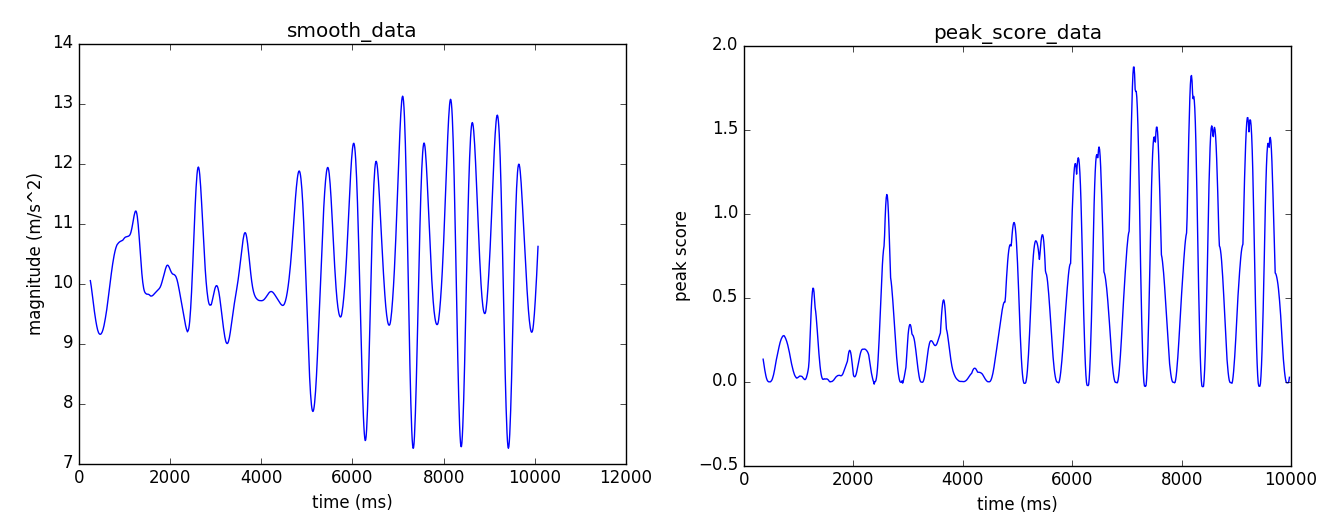
\includegraphics[width=\textwidth]{Images/max_diff_score.png}
                    \centering
                    \caption{Peak Scoring using Maximum Difference with $N=6$. Filtered data is on the left, smoothed data is on the right. Note how the large peaks are amplified, while the smaller ones are suppressed.}
                    \label{max_diff_score}
                \end{figure}                 

            \subsection{Mean Difference}

                This method is similar to Maximum Difference, except that instead of taking the maximum of the difference to the left and the right, Mean Difference takes the mean of all the differences. The effect is similar to Maximum Difference, but smaller in magnitude. It also preserves the overall shape of the waveform.

                An example of the output from a filtered signal to the scored signal using Mean Difference is shown below in Figure \ref{mean_diff_score}.

                The equation describing this behavior is given by:

                \begin{equation}
                x = \frac{\sum_{k=-N, k\neq i}^{N} (x_i - x_{i+k})}{2N},
                \end{equation}

                where $i$ is the point under consideration, $x_n$ is the value of the signal at the $n^{th}$ sample, and $N$ is the characteristic length of the Mean Difference operation.

                \begin{figure}[!th]
                    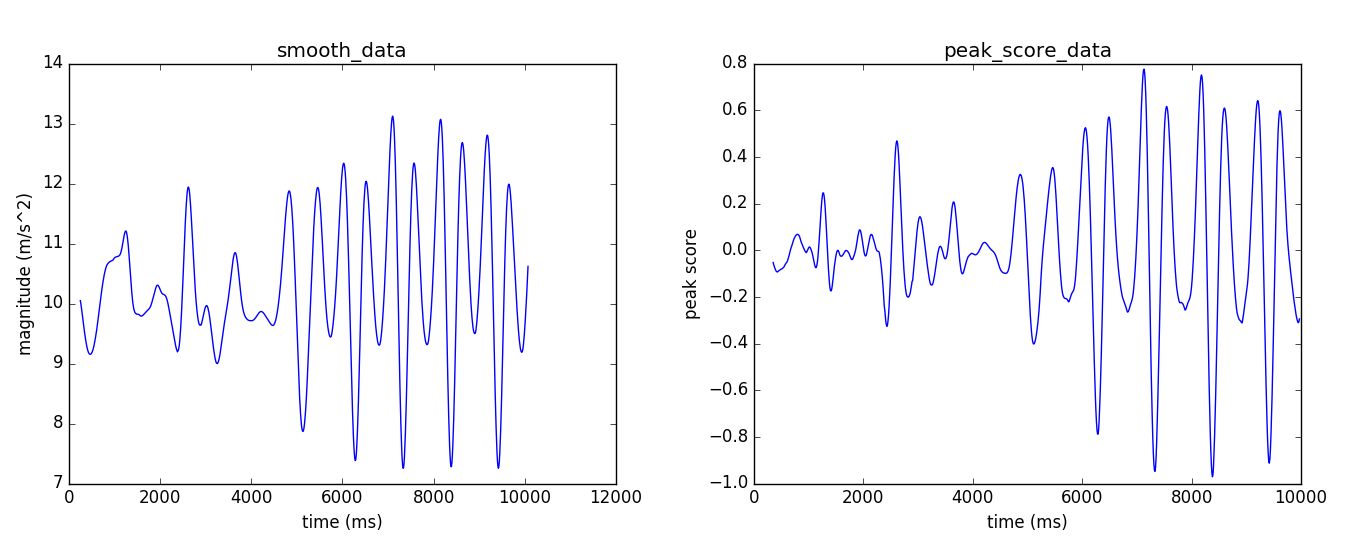
\includegraphics[width=\textwidth]{Images/mean_diff_score.png}
                    \centering
                    \caption{Peak Scoring using Mean Difference with $N=10$. Filtered data is on the left, scored data is on the right.}
                    \label{mean_diff_score}
                \end{figure}

            \subsection{Modified Pan-Tompkins Scoring}

                This method is a derivative from the famous algorithm by Pan and Tompkins [CIT] that was used for peak detection. 

                The original algorithm had four main steps: digital bandpass filter, differentiate the signal, square the signal, then a moving integration window to reconstitute the signal.

                From this baseline, a modified algorithm was developed:

                \begin{itemize}
                    \item Locally zero-mean the data around with a window of size $N$.
                    \item Set all the data points that are less than 0 to zero.
                    \item Square the data to amplify any large peaks.
                \end{itemize}

                The first step is integral as it ensures that when the data is squared, only truly large peaks get amplified. The second step is important to ensure that only positive peaks get detected. Without this, the algorithm would detect both the peak and trough.

                An example of this scoring using this method is shown below in Figure \ref{pan_tompkins_score}.

                \begin{figure}[!th]
                    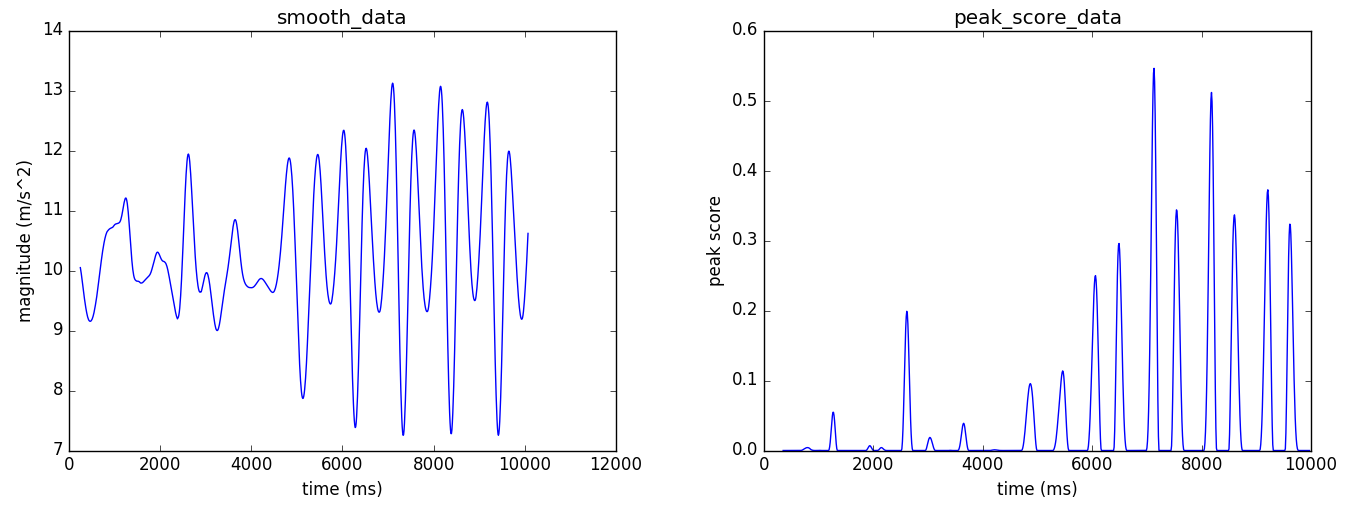
\includegraphics[width=\textwidth]{Images/pan_tompkins_score.png}
                    \centering
                    \caption{Peak Scoring using Modified Pan-Tompkins with $N=10$. Filtered data is on the left, scored data is on the right.}
                    \label{pan_tompkins_score}
                \end{figure}


        \section{Detection Stage}

            The next stage in the process is to identify potential candidates for peaks associated with peaks. This is done using statistics to identify outliers. 

            As the algorithm traverses the signal, it keeps track of a running mean and standard deviation. Computationally efficient way of doing this incrementally are as shown below:

            \begin{equation}
                \bar{x}_n = \frac{x_n + (n-1)\bar{x}_{n-1}}{n},
            \end{equation}

            \begin{equation}
                \sigma_n^2 = \frac
                {(n-2)\sigma_{n-1}^2 + (n-1)(\bar{x}_{n-1} -\bar{x}_n)^2 + (x - \bar{x}_n)^2}
                {n-1},
            \end{equation}

            where $x_n$ is the $n^{th}$ sample, $\bar{x}_n$ is the running mean at the $n^{th}$ sample, and $\sigma_n$ is the running standard deviation at the $n^{th}$ sample.

            The algorithm will then use these two quantities to determine whether any given point is an outlier by thresholding. That is to say, if a point is $c$ or more running standard deviations above the running mean, then it is marked as a potential peak.

            \begin{equation}
                \frac{x_n - \bar{x}_n}{\sigma_n} \stackrel{?}{\geq} c,
            \end{equation}

            where $c$ is the designated threshold.

            An example of the results of this method is shown below in Figure \ref{img_detection_stage}.

            Note that the algorithm skips a number of points at the beginning as it builds up a running mean and standard deviation. Unfortuntely, this means that, almost always, the first peak it encounters will be marked as a potential step.

            \begin{figure}[!th]
                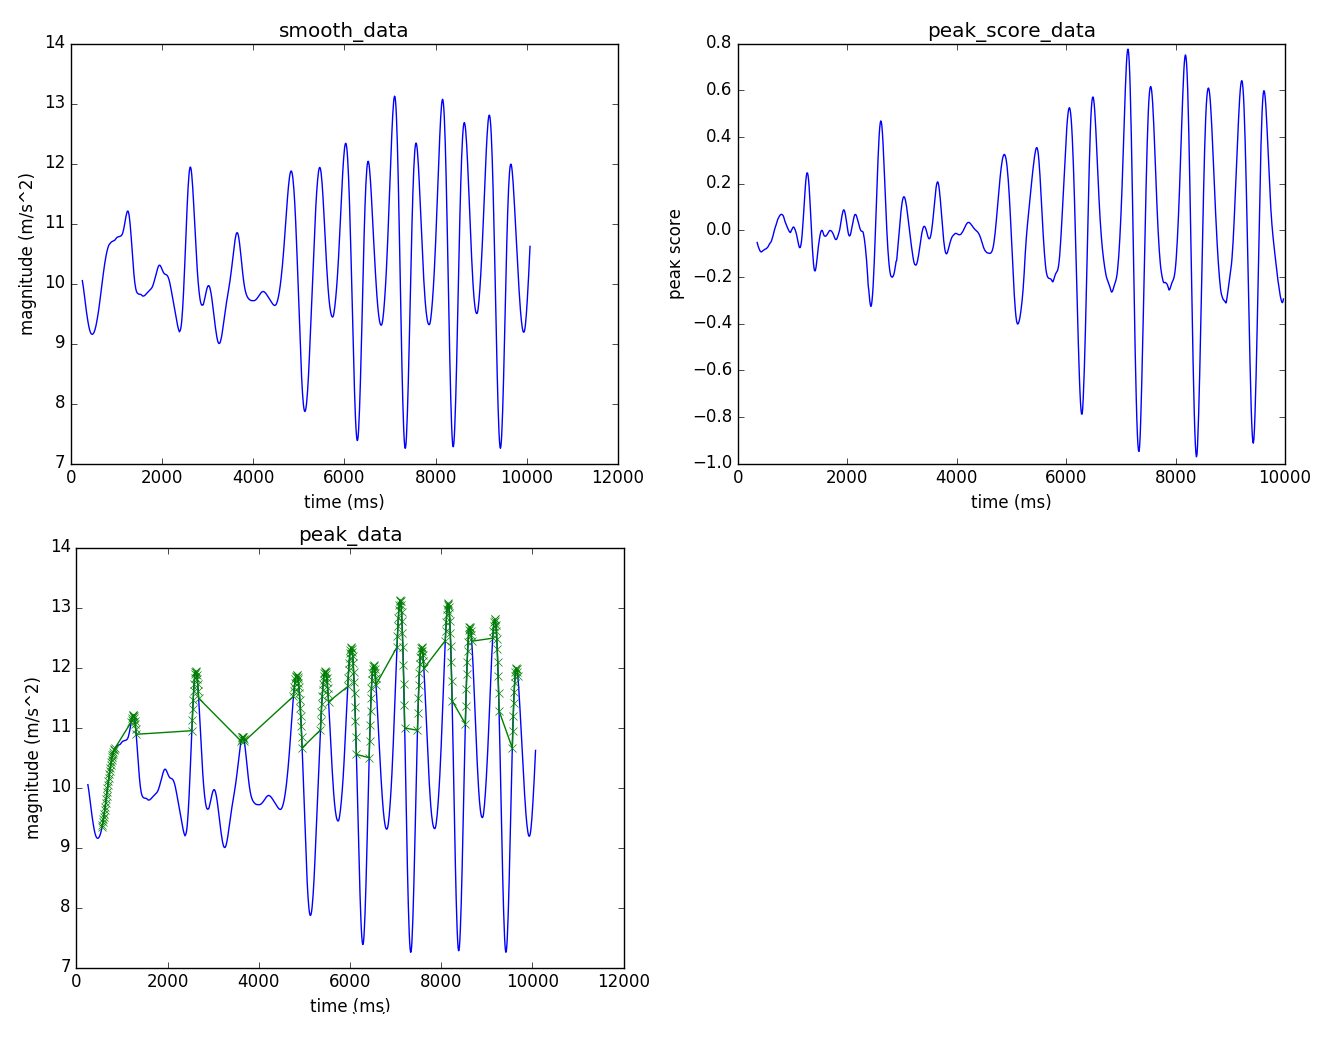
\includegraphics[width=\textwidth]{Images/detection_stage.png}
                \centering
                \caption{The results of the Peak Detection stage. Top Left: filtered signal, Top-Right: scored signal, Bottom-Left: filtered signal with potential peaks overlaid in green. $c=1.2$ for the Peak Detection stage.}
                \label{img_detection_stage}
            \end{figure}

        \section{Post-Processing Stage}

            The final stage of the algorithm is to collect the potential peaks from the previous stage and clean these such that only the true peaks remain. In Figure \ref{img_detection_stage}, all of the potential peak points are clustered on the rise to the peak, this stage should remove all the erroneous points and leave only the maximum of each peak. This stage also makes use of the fact that the peaks associated with walking are usually periodic with a minimum delay between them. Note this delay is related to the speed of walking.

            This stage moves a window of a fixed size, $t_{window}$, across the potential peaks and only keeps the maximum point in the window. This effectively removes all the points leading up to the peak while preserving the peak. By tuning the window size, the algorithm can ensure that for most cases no two steps will reside in this window at the same time. This window was set to $200ms$ which translates to a maximum walking speed of $5 steps/sec$, far faster than average walking pace.

            The pseudocode for such an operation would be like the following:

            \begin{lstlisting}
int windowSize = 200; // In ms
Point currentMax;
// Iterate through the sorted list of points
for (Point candidate in points) {
    if (candidate.time - currentMax.time > windowSize) {
        // The currentMax point is now outside the window. 
        yield currentMax;
        currentMax = candidate;
    } else {
        // Keep the maximum point.
        currentMax = (currentMax.value > candidate.value) ? currentMax : candidate;
    }
}
            \end{lstlisting}

            The result of this simple operation retains the peak points while throwing away the points surrounding the peak, this is exactly the intended behavior. An example of this can be seen in \ref{img_post_stage}.

            \begin{figure}[!th]
                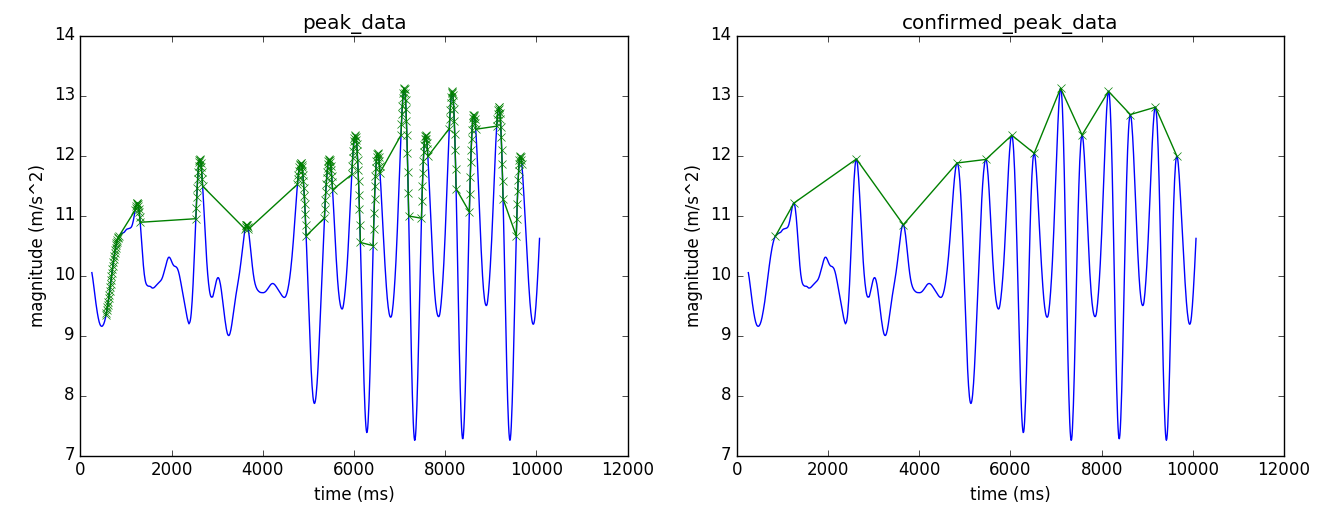
\includegraphics[width=\textwidth]{Images/post_stage.png}
                \centering
                \caption{The results of the Post-Processing Stage. Output of the Detection Stage is on the left, output of the Post-Processing Stage is on the right. Note how the set of points surrounding the peaks have been filtered out.}
                \label{img_post_stage}
            \end{figure}

    \chapter{Data Collection Apparatus}

        A dataset with ground truth data must be acquired in order to optimize and validate the algorithm. The algorithm is only interested in the overall accuracy over periods of time, so a simple total count of steps is all that is required. However, in order to open up the versatility of the dataset and enable future improvements of the algorithm, a dataset was collected that would also contain the information for timestamps of the steps with the ground truth. Note that the total count of steps can easily be obtained from this more detailed dataset. 

        Previous studies, such as [CIT], used video annotation to determine the time stamps of steps, but this is time intensive and prone to error and human inaccuracy. In order to accurately determine this information, a custom device had to be designed and built.

        \section{Custom Design}

            The device is designed to record steps with some sort of sensor attached to the shoe. The sensors are connected to an RFduino, which is a Bluetooth-enabled Arduino microcontroller board. The RFduino will poll the sensor for information and broadcast it over Bluetooth Low Energy to an Android smartphone, discussed later. 

            The first iteration of the device used push buttons mounted on straps that would be strapped around the vamp of the shoe, covering the ball of the user's foot. These push buttons would be connected to the RFduino with a simple pull down resistor, such that logic level 0 indicates that the push button is up and the user's foot is up and logic level 1 indicates that the push button is down and the user's foot is down. A picture of the push button mounted on the straps can be seen below in Figure \ref{img_device_og} along with a picture of the device in use in Figure \ref{img_device_og_use}.

            \begin{figure}[!th]
                \includegraphics[width=0.6\textwidth]{Images/device_og.jpg}
                \centering
                \caption{A picture of the original ground truth device design. Note the push button in the middle of the pink strap. The contact area was reinforced with cardboard in an attempt to increase robustness.}
                \label{img_device_og}
            \end{figure}

            \begin{figure}[!th]
                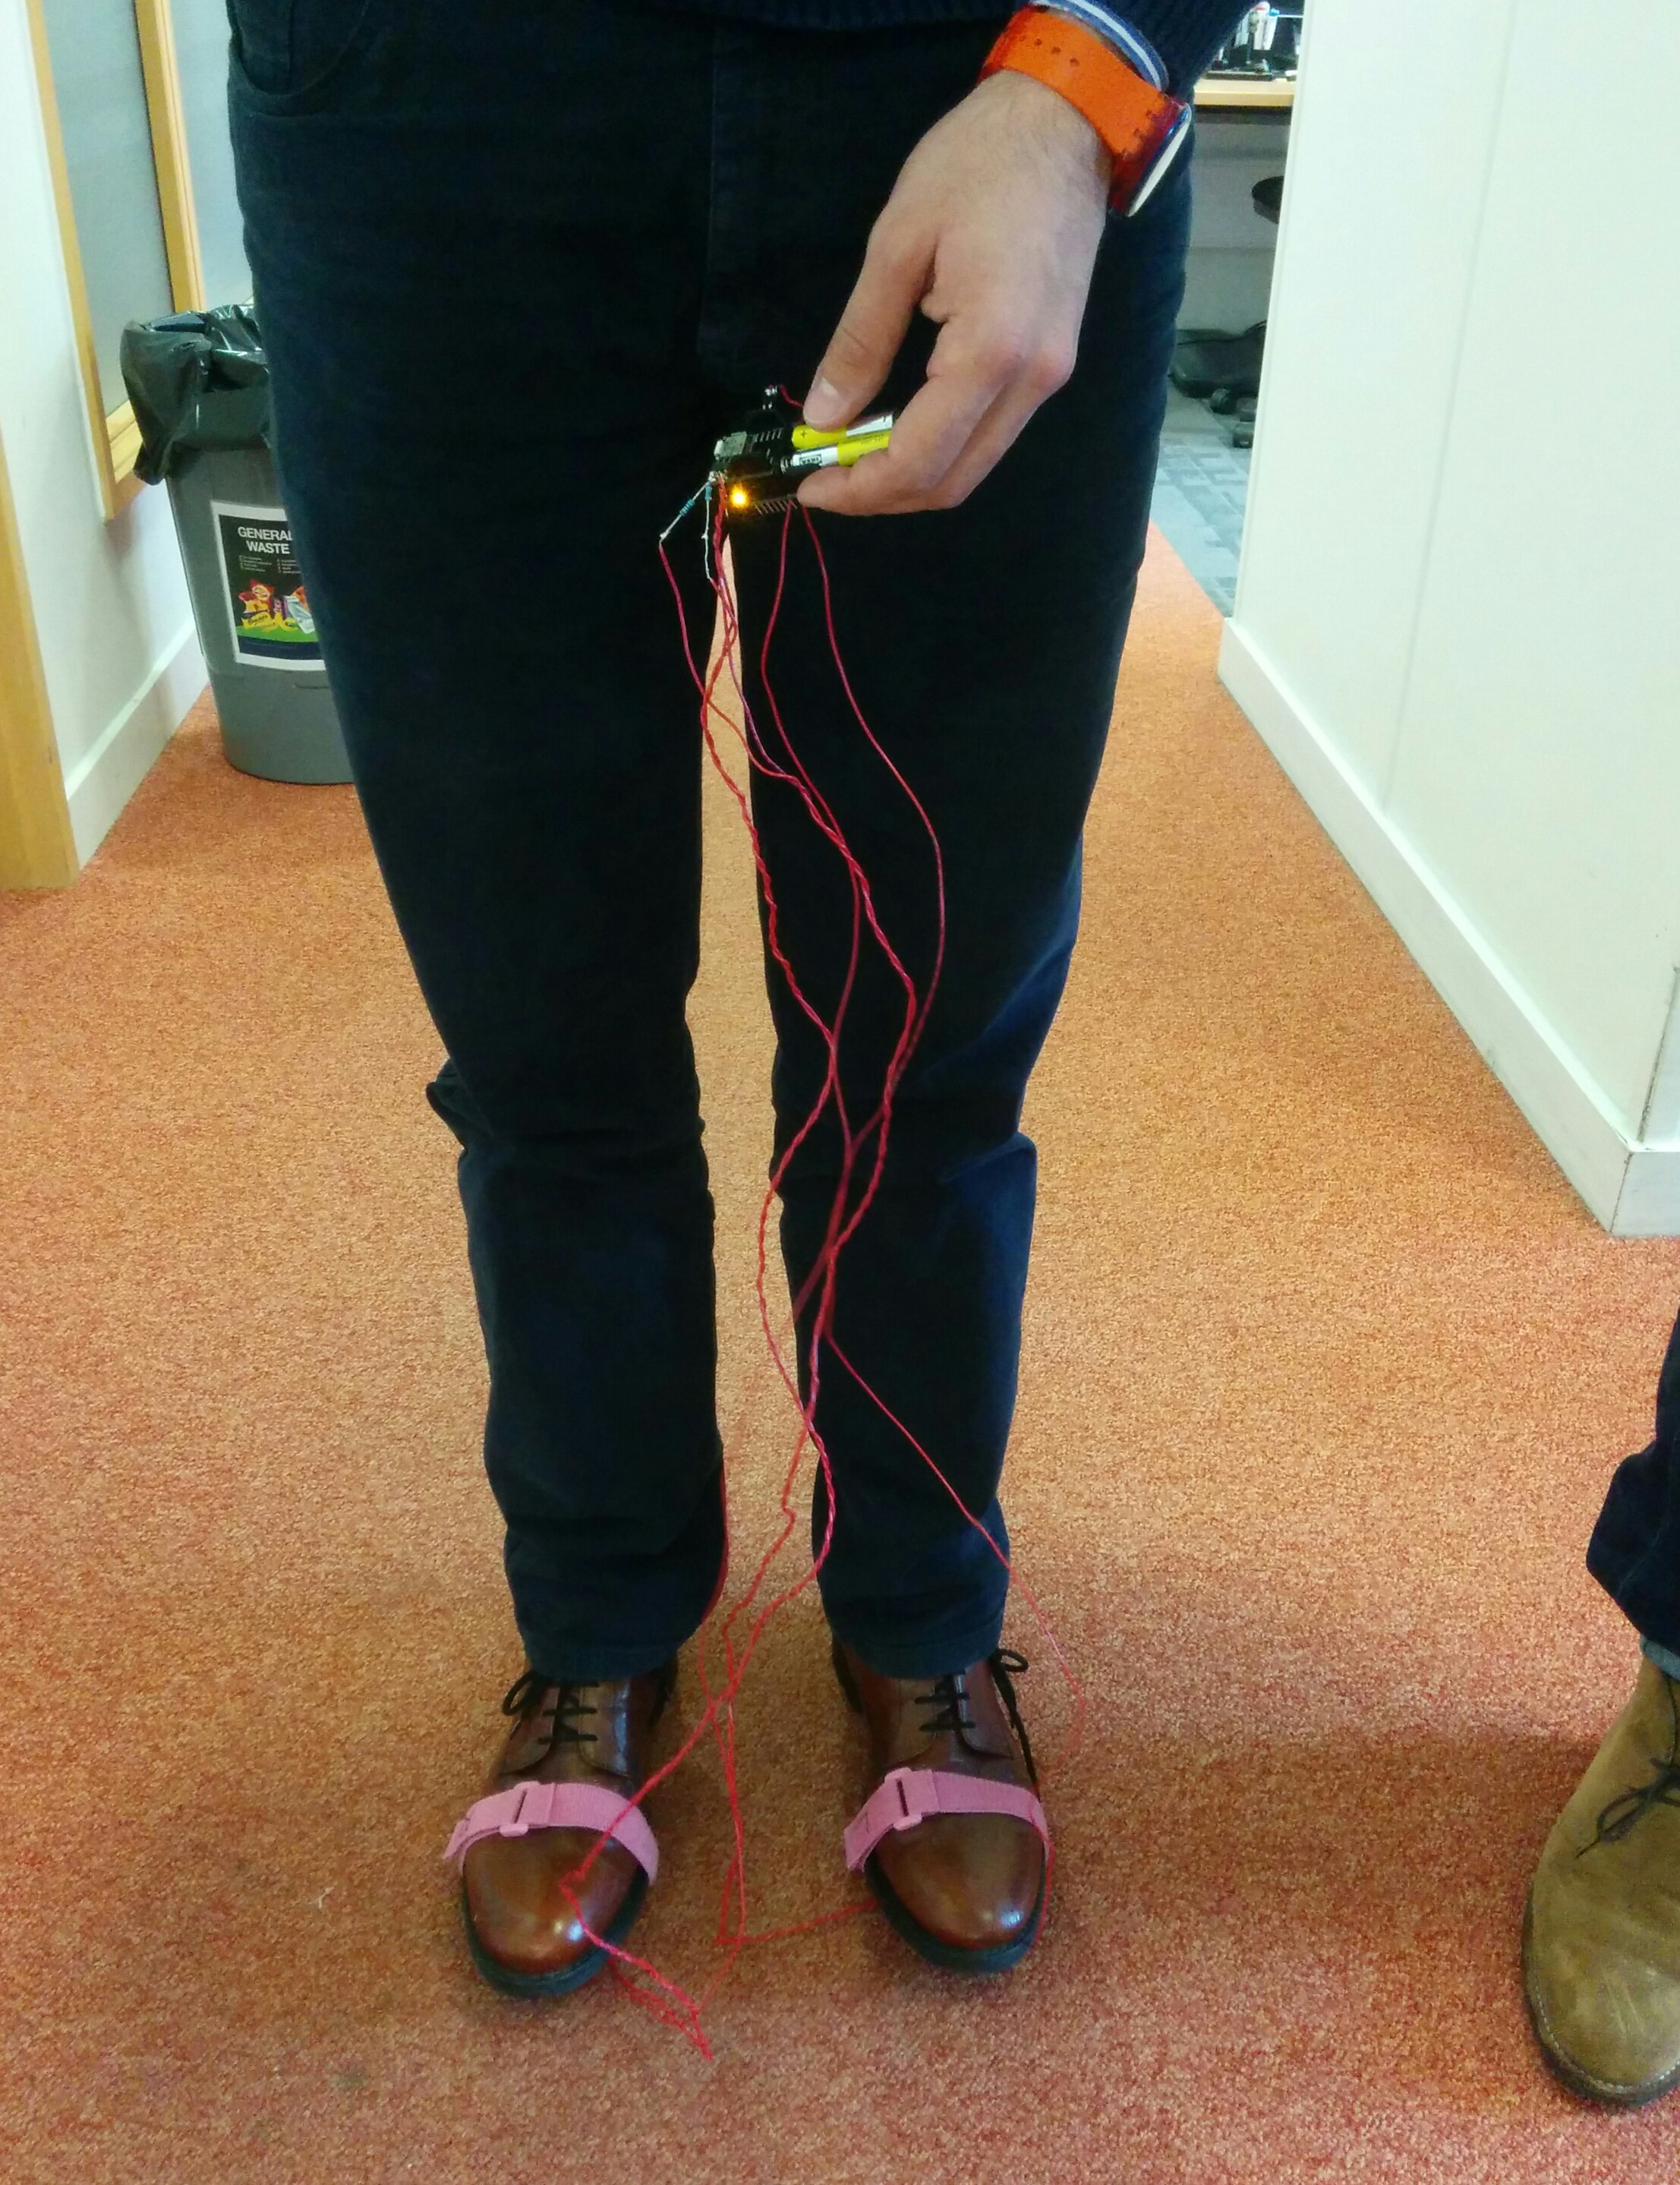
\includegraphics[width=0.6\textwidth]{Images/device_og_use.jpg}
                \centering
                \caption{A picture of the original ground truth device in use. Notice the placement of the straps on the user's shoes such that the push button would be positioned roughly under the ball of the foot.}
                \label{img_device_og_use}
            \end{figure}

            Unfortunately, this iteration of the device was subject to a number of problems regarding robustness. The device worked well when functional, but it suffered from the breaking of the push buttons due to excessive force. The pins of the push buttons also broke a number of times as they were folded flat against the strap due to the weight of the user. Clearly, a more robust design was required.

            The second iteration of the design dropped the push buttons entirely and moved to a method that relied on having a pressure sensitive resistor sit under the heel of the user inside the shoe. To ensure that this resistor is tolerant and sensitive to the relatively high pressures in this use case, the device used a material called velostat as the variable resistor. Velostat, used primiarly as a packaging material, is "made of polymeric foil impregnated with carbon black to make it electrically conductive" [CIT]. The resistance is reduced when pressure is applied, hence when current flow is high, the foot is down. The new device was made by taping conductive thread to either side of the velostat, completing the circuit. A picture of the new device can be seen in Figure \ref{img_device_new}.

            \begin{figure}[!th]
                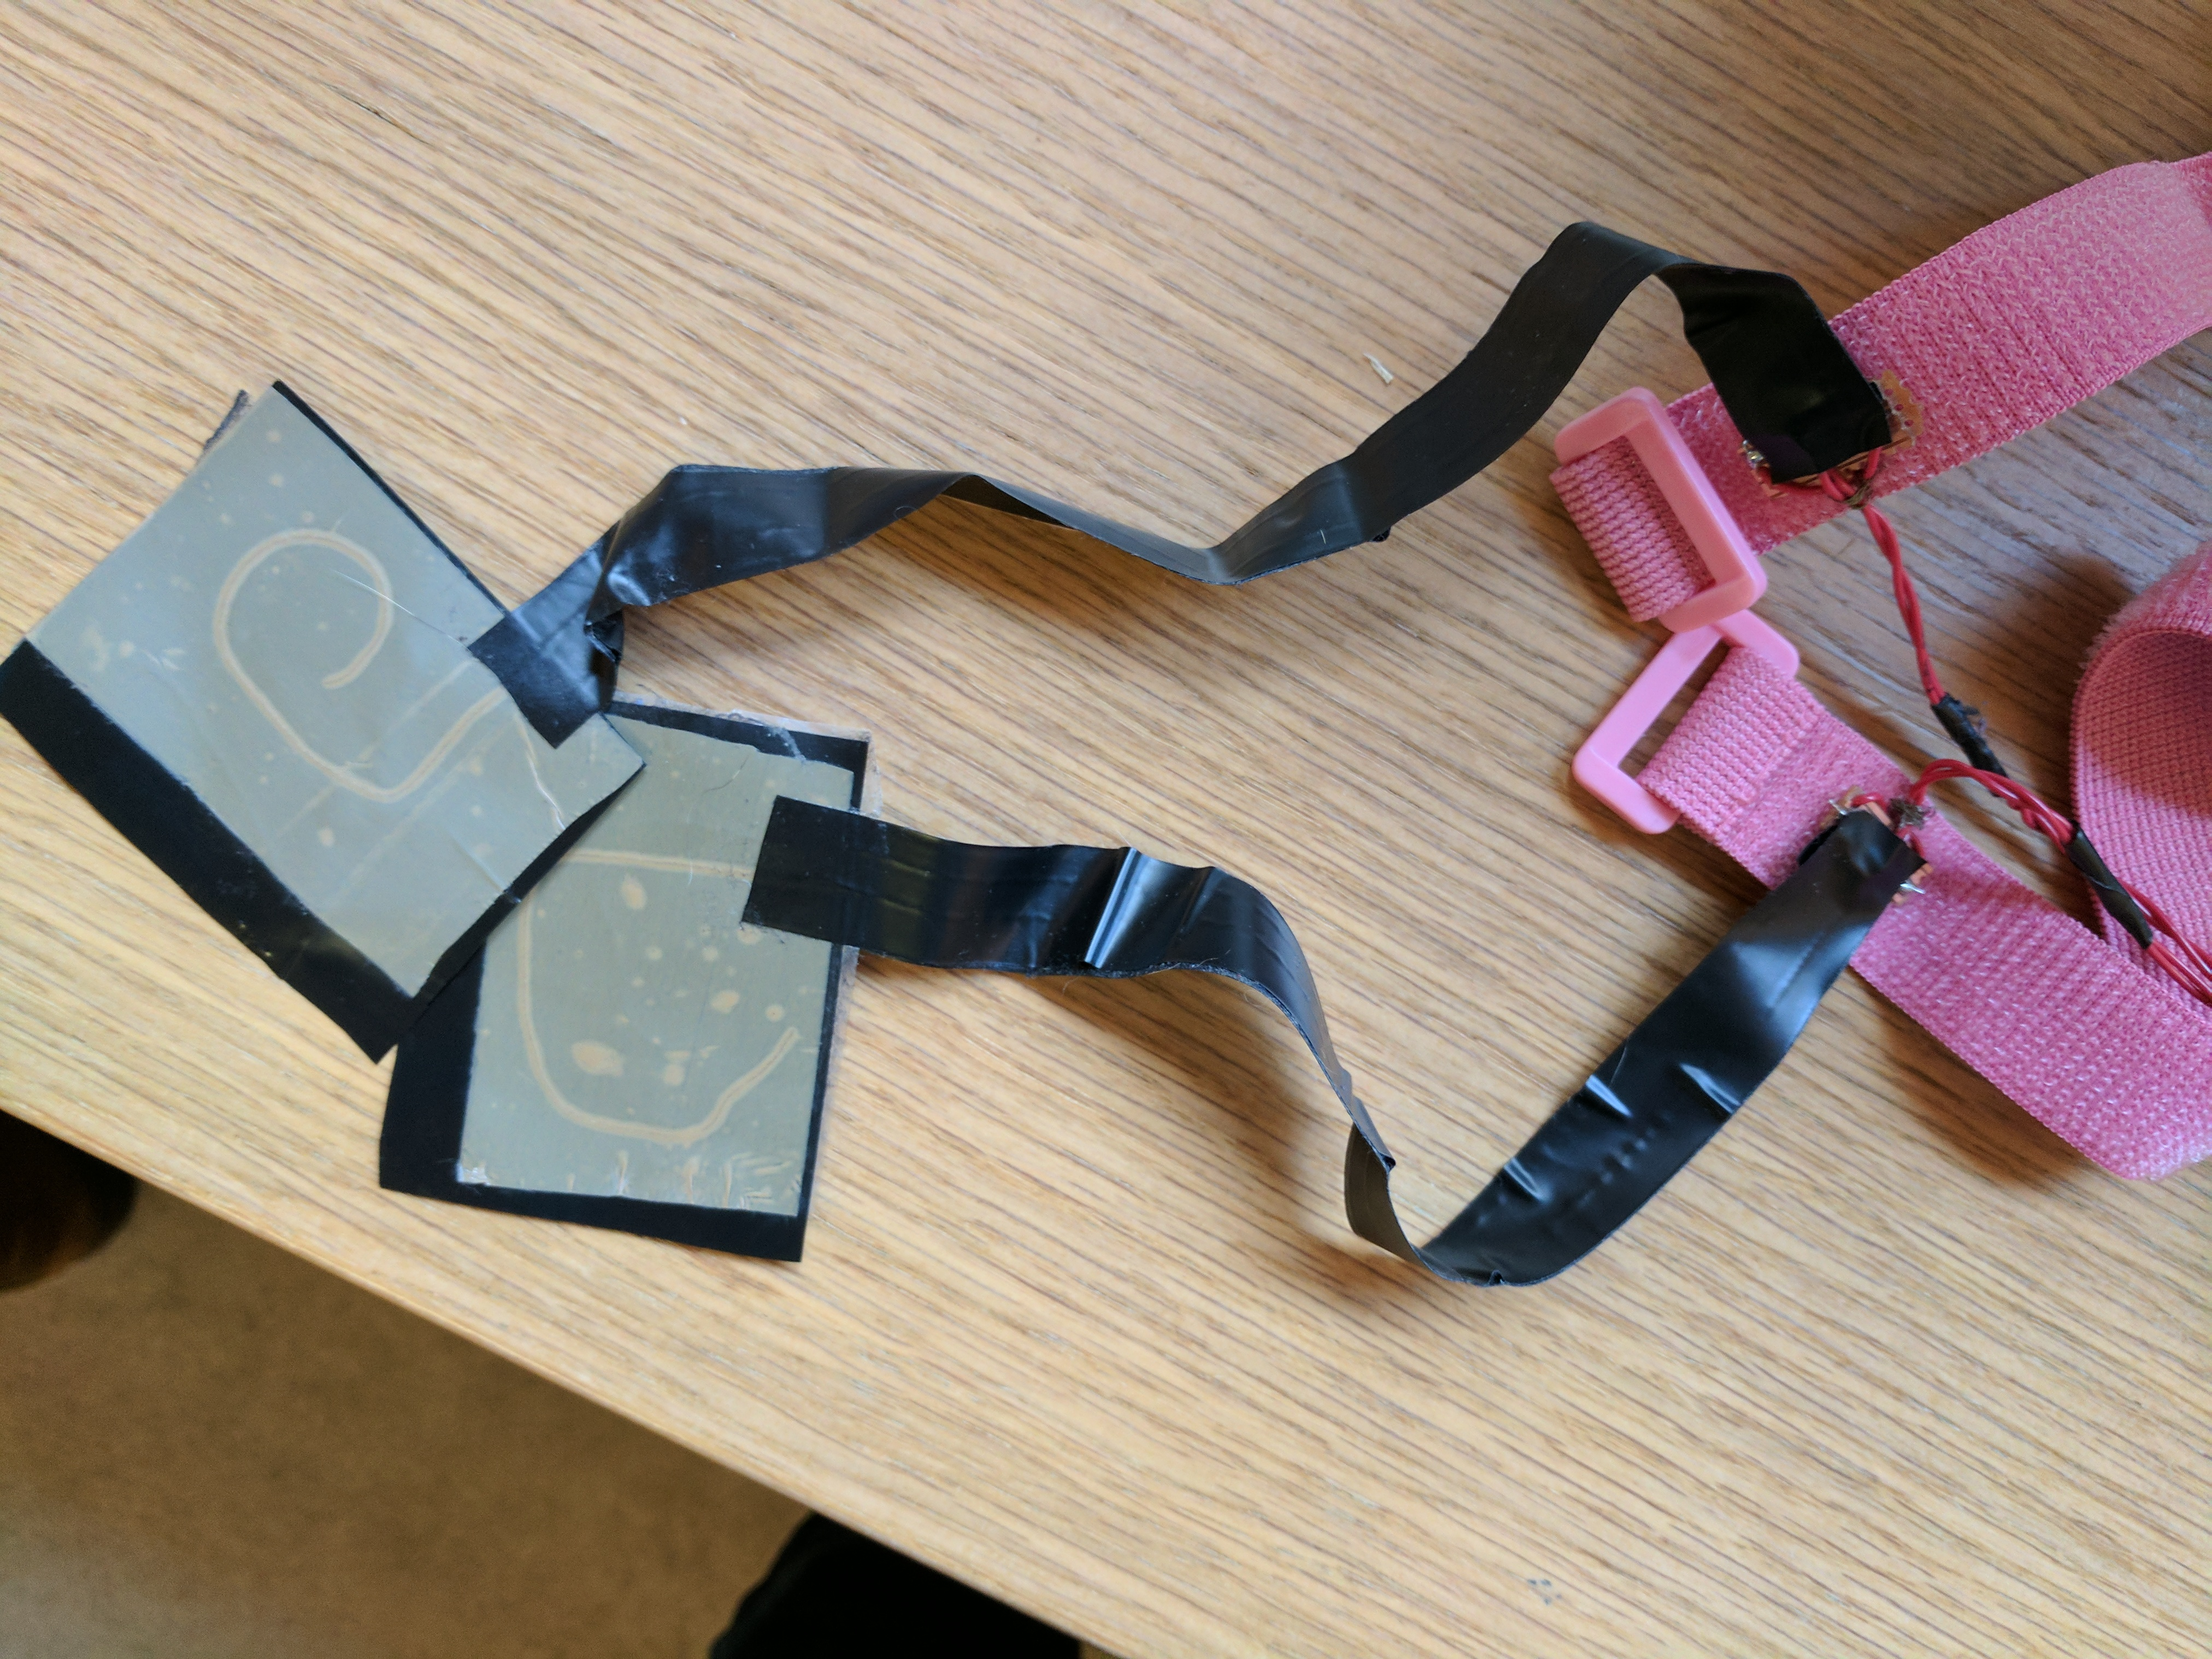
\includegraphics[width=0.6\textwidth]{Images/device_new.jpg}
                \centering
                \caption{The new ground truth device. Note the conductive thread visible through the tape and the electrical tape used to keep the two threads electrical isolated. The straps would now be put around the user's ankles.}
                \label{img_device_new}
            \end{figure}

            The firmware on the RFduino uses a moving threshold to determine the on-off switch point. The threshold for each sensor is calculated by retaining a history of the minimum and maximum values of each sensor, and then taking the midpoint of the min and max. Every 5 seconds, the minimum and maximum are penalised such as to ensure that exceptionally low or high results long ago do not fix the min and max for the entire trace. A graph representing the raw data from the sensors plotted against the thresholds is shown below in Figure \ref{img_device_new_graph}.

            \begin{figure}[!th]
                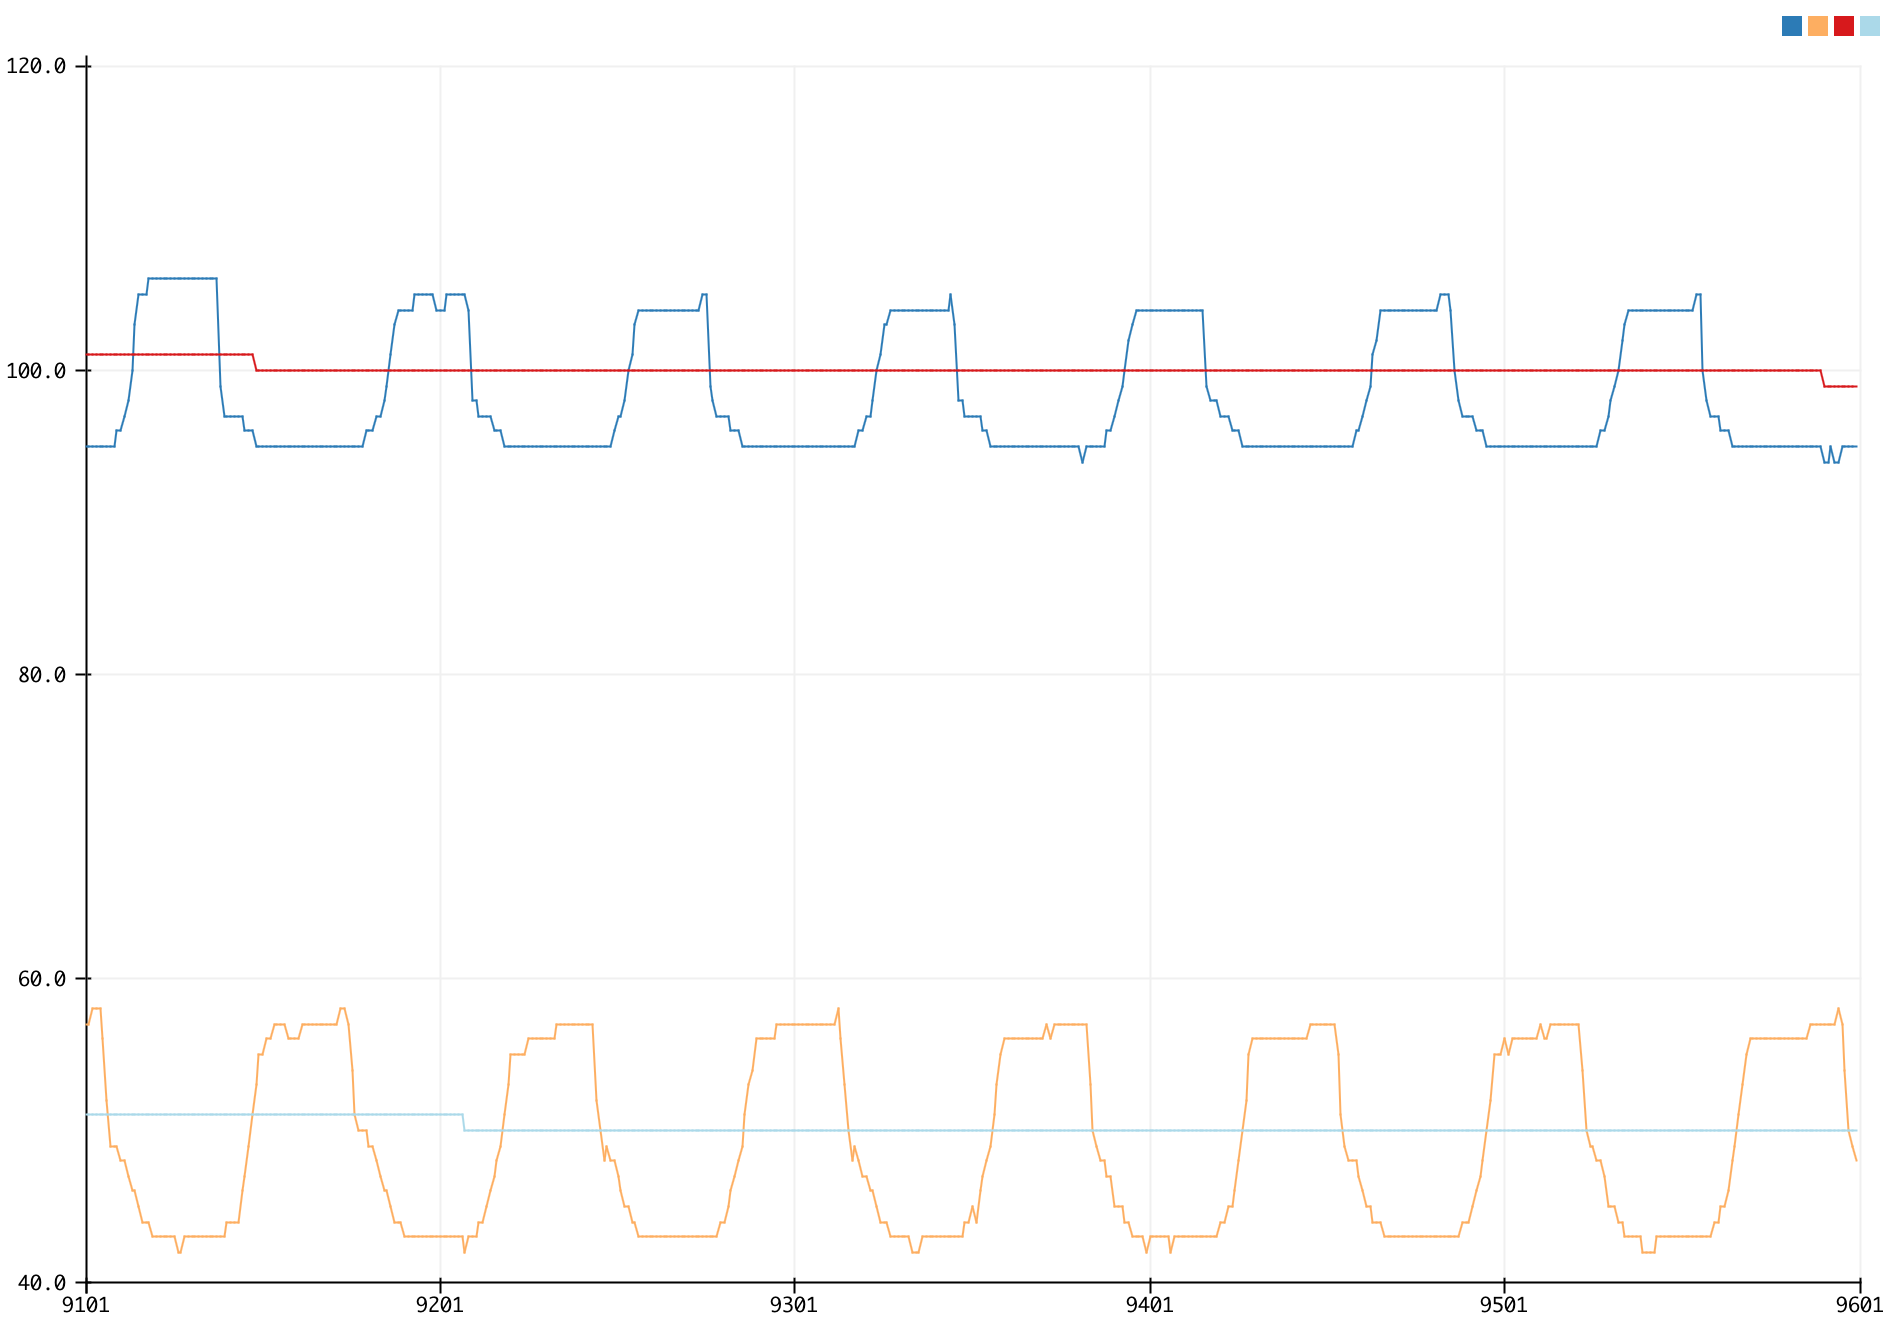
\includegraphics[width=0.8\textwidth]{Images/device_new_graph.png}
                \centering
                \caption{The raw data captured by the new ground truth device. Note how the steps are clearly discernable and the moving threshold correctly classifies the two states. The difference in magnitude for each signal is explained by the natural variation in velostat pads.}
                \label{img_device_new_graph}
            \end{figure}         


        \section{Android Application}

            To capture the accelerometer data and the ground truth simultaneously, an Android application had to written to accomodate this functionality. It had to:

            \begin{itemize}
                \item Capture accelerometer data at a high rate (at least 100Hz) and save to a file.
                \item Connect via Bluetooth Low Energy to the ground truth device, decode the signal, and save the data to a file with synchronized timestamps with respect to the accelerometer data.
                \item Provide a simple method of retrieving this data off the device.
                \item Provide a simple UI for the user to capture all of this data efficiently.
            \end{itemize}

            For expendiency's sake, application was designed such that the data would be zipped and compressed together and uploaded to a remote server via HTTP POST. This enabled the user to record mulitple data recordings after one another without needing to manually retrieve the files off the device.


        \section{Dataset}

            As the algorithm should be able to run well over a myriad of scenarios, a dataset was collected that aimed to encapsulate as many of these scenarios as possible. The dataset features 3 people collecting data with a variety of heights and weights, 3 phones to ensure that similar devices performed similarly, and 6 phone 'positions': in a hand, in a front pocket, in a back pocket, in an armband, in a shoulder purse, and in a neck pouch on a lanyard. 

            This resulted in a dataset containing 48 distinct traces, each with approximately $2.5$ minutes of accelerometer and ground truth data. This dataset should provide a good range of scenarios for optimization such that the final algorithm parameters will be the best performing averaged over a variety of scenarios. It also opens the possibility of specific parameter combinations that provide very high accuracy for a specific scenario. 

            In addition, 3 data traces were collected from current patients in the ?? without the ground truth device data for post-optimization validation. The total step counted was instead hand counted by a trainer professional present at the recording.

    \chapter{Algorithm Optimization}

        Now that the algorithm and it's parameters have been described and that the dataset and the method by which it was collected was described, the optimization of the algorithm can be described. This can be generalized as a maxization problem where the domain of the problem is defined by the parameter space. The only certain way of getting a guaranteed maximum is to run a search across the parameter space. Each stage may have parameters associated with it, and these parameters may change depending on the stage selection (choice of filter, scoring technique). 

        In order to keep the running time of the optimization routine to a reasonable limit, this parameter search will need to be fairly rough to limit the number of parameter permutations. By manually testing extremes of the parameters, the set of parameters to test can be reduced to a more reasonable set. The final set can be seen in Tables \ref{tbl_filtering}, \ref{tbl_scoring}, \ref{tbl_detection}. Note that the first stage, Pre-Processing, has been held constant at $t_{scale}=10^6$ and $f_{int}=100Hz$. The Post-Processing stage has also been held constant at $t_{window}=200ms$. 


        \begin{center}
            \captionof{table}{The parameter set for the Filtering Stage.}
            \label{tbl_filtering}
            \begin{tabular}{|c|c|c|c|}
                \hline
                Parameter & Minimum & Step & Maximum \\
                \hline
                \multicolumn{4}{|c|}{\textbf{Moving Average Filter}} \\
                \hline
                Window Size ($N$) & 13 & 8 & 53 \\
                \hline
                \multicolumn{4}{|c|}{\textbf{Hann Filter}} \\
                \hline
                Window Size ($N$) & 13 & 8 & 53 \\
                \hline
                \multicolumn{4}{|c|}{\textbf{Gaussian Filter}} \\
                \hline
                Window Size ($N$) & 13 & 8 & 53 \\
                Standard Deviation ($\sigma$) & 0.35 & Fixed & 0.35 \\
                \hline
                \multicolumn{4}{|c|}{\textbf{Kaiser-Bessel Filter}} \\
                \hline
                Window Size ($N$) & 13 & 8 & 53 \\
                Sampling Frequency ($f_s$) & 100Hz & Fixed & 100Hz \\
                Cutoff Frequency ($f_c$) & 3Hz & Fixed & 3Hz \\
                Drop At $f_c$ ($A$) & 60dB & Fixed & 60dB \\
                \hline
            \end{tabular}
        \end{center}

        \begin{center}
            \captionof{table}{The parameter set for the Scoring Stage.}
            \label{tbl_scoring}
            \begin{tabular}{|c|c|c|c|}
                \hline
                Parameter & Minimum & Step & Maximum \\
                \hline
                \multicolumn{4}{|c|}{\textbf{Maximum Difference}} \\
                \hline
                Window Size ($N$) & 3 & 8 & 51 \\
                \hline
                \multicolumn{4}{|c|}{\textbf{Mean Difference}} \\
                \hline
                Window Size ($N$) & 3 & 8 & 51 \\
                \hline
                \multicolumn{4}{|c|}{\textbf{Modified Pan Tompkins}} \\
                \hline
                Window Size ($N$) & 11 & 8 & 51 \\
                \hline
                \multicolumn{4}{|c|}{\textbf{No Scoring Method}} \\
                \hline
                \multicolumn{4}{|c|}{No Parameters} \\
                \hline
            \end{tabular}
        \end{center}
        \begin{center}
            \captionof{table}{The parameter set for the Detection Stage.}
            \label{tbl_detection}
            \begin{tabular}{|c|c|c|c|}
                \hline
                Parameter & Minimum & Step & Maximum \\
                \hline
                Standard Deviation Threshold ($c$) & 1.2 & 0.2 & 1.4 \\
                \hline
            \end{tabular}
        \end{center}

        These parameter variations give the total number of permutations at 1008. Each of these parameter sets will be tested on all 48 data recordings listed in the previous section. The results will be averaged across all data recordings for each permutation to give a general accuracy rating. This will be the variable upon which the optimal set will be decided. 

        However, since there are approximately $2$ hours of data to run through the algorithm, each permutation test takes a bit of time. Specifically, on a machine with an Intel i5-6200u, it takes about $5$ minutes for each. This means that if this optimization were to run solely on that machine, it would take $3.5$ days to complete! 

        The solution to this problem is to build a distributed computing platform such that the computing load can be spread across multiple workers. To ensure that each parameter set only gets computed once, there will be a central server that is in charge of distributing parameter sets to each of the workers. 

        This backend server was built on Flask [CIT], a microframework for Python, and served over gunicorn [CIT], a Python WSGI (Web Server Gateway Interface) HTTP webserver. The data would be passed back and forward via JSON. The backend would also store the results in a Postgres SQL (Structured Query Language) database [CIT] such that the results can be queried easily.

        Each worker would have an implementation of the algorithm and the dataset locally. The worker will query the backend for a new set of parameters, and fetch the JSON of these with an HTTP GET request. When the computation is completed, the worker will append the results to the JSON file and return it via an HTTP POST request to the backend. It would then request a new set of parameters, until all permutations have been exhausted.

        In this instance, Google Cloud Compute [CIT] was used to spin up 8 workers to run the algorithm, such that the runtime of the routine was cut down to around 11 hours. This is much more manageable and reasonable!

    \chapter{Results}

        \section{Optimal Parameters}

            The best set of parameters given by the optimization routine given above achieved an average accuracy of 93.7\% across the 48 data recordings. The parameters that achieve this accuracy is given by Table \ref{tbl_opt_params}.

            \begin{center}
                \captionof{table}{The parameters for the optimal algorithm performance.}
                \label{tbl_opt_params}
                \begin{tabular}{|c|c|c|}
                    \hline
                    Stage & Type & Parameters \\
                    \hline
                    Pre-Processing & Default & $t_{scale}=10^6$, $f_{int}=100Hz$ \\
                    Filtering & Gaussian & $N=13$, $\sigma=0.35$ \\
                    Scoring & Mean Difference & $N=27$ \\
                    Detection & Default & $c=1.2$ \\
                    Post-Processing & Default & $t_{window}=200ms$ \\
                    \hline
                \end{tabular}
            \end{center}

            The spread of the accuracy results can be seen below in Figure \ref{img_opt_params_overall}. This shows that the majority of the accuracy results is within the 90\% to 100\% range with some outliers showing significantly lower accuracy.

            \begin{figure}[!th]
                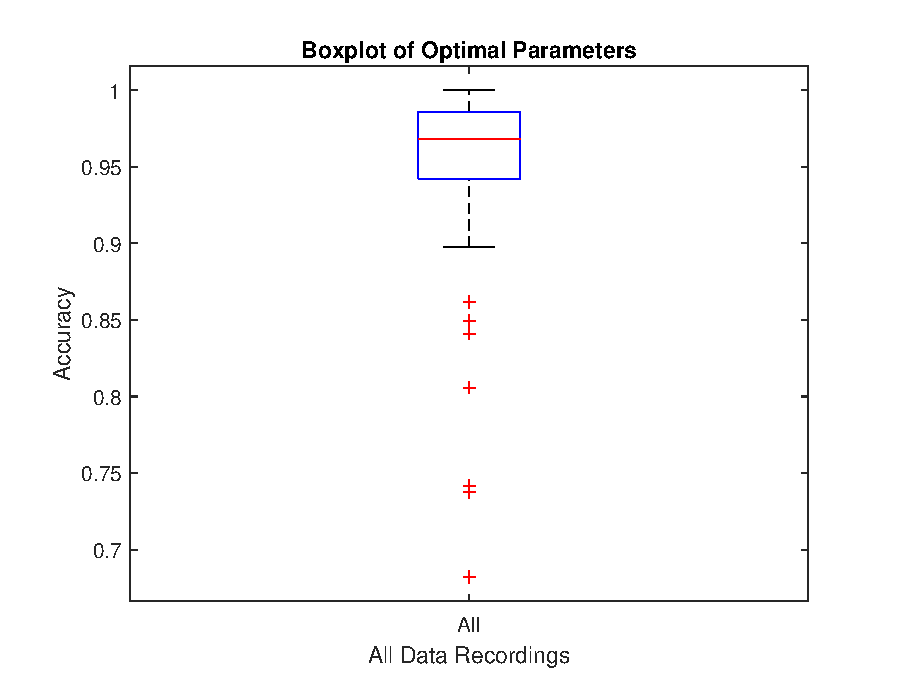
\includegraphics[width=0.8\textwidth]{Images/opt_params_overall.eps}
                \centering
                \caption{The spread of the accuracy of the optimal parameters over the 48 data recordings.}
                \label{img_opt_params_overall}
            \end{figure}

            If the results are split by the position the phone was in when the data was recorded, the source of these outliers can be seen. These plots can be seen below in Figure \ref{img_opt_params_positions_bp}.

            \begin{figure}[!th]
                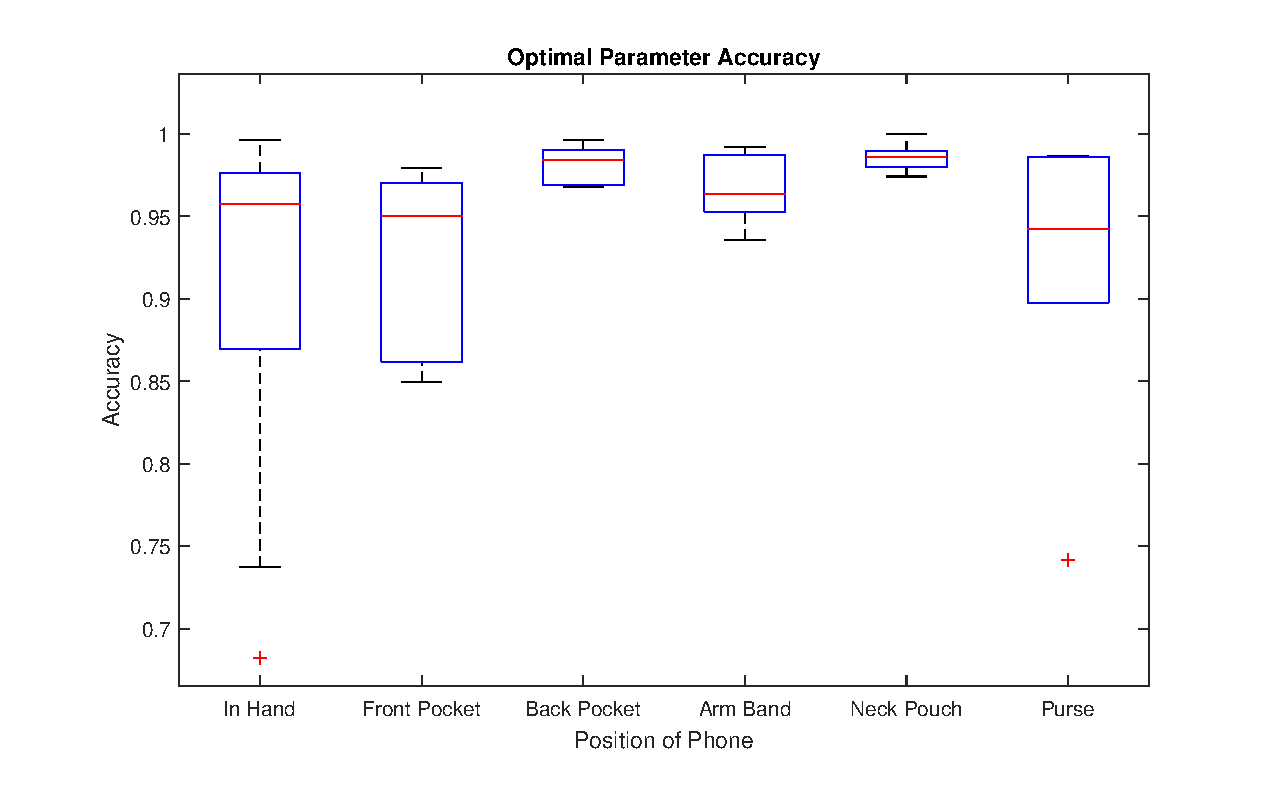
\includegraphics[width=0.8\textwidth]{Images/opt_params_positions_bp.eps}
                \centering
                \caption{The spread of the accuracy of the optimal parameters over the 48 data recordings grouped by phone position. The far outliers overwhelmingly come from the 'In Hand' position.}
                \label{img_opt_params_positions_bp}
            \end{figure}

            As can be seen from Figure \ref{img_opt_params_positions_bp}, the outliers come primarily from the 'In Hand' or 'Purse' positions. This leads to the hypothesis that these positions may induce some harmonics in the walking frequency range that are destructive to the signal from stepping. The source of this may be the user swinging their arm when holding the phone or the purse swinging back and forth under arm.

            This grouping also reveals that the 'Back Pocket', 'Arm Band', and 'Neck Pouch' positions seem to be the best positions for the algorithm. It should be noted that the 'Arm Band' may be subject to the same harmonics as the 'In Hand' position, however, the relatively limited movement of the upper arm when compared to the hand limits the impact of these harmonics.

            These parameters can now be validated against the three patient data recordings mentioned earlier too. If the accuracies are similar to the average, then it supports the idea that these parameters are good for a generalized algorithm.

            The results of running these data recordings are detailed below in Table \ref{tbl_patient_results}. The average accuracy of these three tracks is 92.3\%. This is very close to the average accuracy recorded from the 48 data recordings and well within the median quartiles in the boxplot.

            \begin{center}
                \captionof{table}{The results of the optimal parameters for the three patient data recordings.}
                \label{tbl_patient_results}
                \begin{tabular}{|c|c|c|c|}
                    \hline
                    Label & Recorded Number of Steps & Algorithm Output & Accuracy \\
                    \hline
                    Patient 1 & 614 & 654 & 93.5\% \\ 
                    Patient 2 & 567 & 605 & 93.2\% \\
                    Patient 3 & 682 & 749 & 90.2\% \\
                    \hline
                \end{tabular}
            \end{center}

        \section{Position Specific Parameters}

            The investigations above reveals an interesting fact: set of parameters perform differently on different positions. This leads to the idea that the algorithm may be able to swap between parameters given the position of the phone to give the best result. For each position, a set of optimal parameters will be specified. That is to say, if the data is restricted to the data recordings corresponding to just those that have the phone in a given position, which set of parameters give the best performance. This analysis leads to extremely high accuracies for some positions and parameters.

            \subsection{In Hand}

                The best set of parameters for the 'In Hand' position gives an overall accuracy of 92.4\%. The parameters that achieve this are laid out in Table \ref{tbl_params_in_hand}.

                \begin{center}
                    \captionof{table}{The parameters for the optimal algorithm performance in the 'In Hand' position.}
                    \label{tbl_params_in_hand}
                    \begin{tabular}{|c|c|c|}
                        \hline
                        Stage & Type & Parameters \\
                        \hline
                        Pre-Processing & Default & $t_{scale}=10^6$, $f_{int}=100Hz$ \\
                        Filtering & Moving Average & $N=53$ \\
                        Scoring & Mean Difference & $N=11$ \\
                        Detection & Default & $c=1.4$ \\
                        Post-Processing & Default & $t_{window}=200ms$ \\
                        \hline
                    \end{tabular}
                \end{center}

            \subsection{Front Pocket}

                The best set of parameters for the 'Front Pocket' position gives an overall accuracy of 98.0\%. The parameters that achieve this are laid out in Table \ref{tbl_params_front_pocket}.

                \begin{center}
                    \captionof{table}{The parameters for the optimal algorithm performance in the 'Front Pocket' position.}
                    \label{tbl_params_front_pocket}
                    \begin{tabular}{|c|c|c|}
                        \hline
                        Stage & Type & Parameters \\
                        \hline
                        Pre-Processing & Default & $t_{scale}=10^6$, $f_{int}=100Hz$ \\
                        Filtering & Moving Average & $N=29$ \\
                        Scoring & Mean Difference & $N=27$ \\
                        Detection & Default & $c=1.2$ \\
                        Post-Processing & Default & $t_{window}=200ms$ \\
                        \hline
                    \end{tabular}
                \end{center}  

            \subsection{Back Pocket}

                The best set of parameters for the 'Back Pocket' position gives an overall accuracy of 99.2\%. The parameters that achieve this are laid out in Table \ref{tbl_params_back_pocket}.

                \begin{center}
                    \captionof{table}{The parameters for the optimal algorithm performance in the 'Back Pocket' position.}
                    \label{tbl_params_back_pocket}
                    \begin{tabular}{|c|c|c|}
                        \hline
                        Stage & Type & Parameters \\
                        \hline
                        Pre-Processing & Default & $t_{scale}=10^6$, $f_{int}=100Hz$ \\
                        Filtering & Gaussian & $N=21$, $\sigma=0.35$ \\
                        Scoring & No Scoring & \\
                        Detection & Default & $c=1.2$ \\
                        Post-Processing & Default & $t_{window}=200ms$ \\
                        \hline
                    \end{tabular}
                \end{center}

            \subsection{Arm Band}

                The best set of parameters for the 'Arm Band' position gives an overall accuracy of 99.4\%. The parameters that achieve this are laid out in Table \ref{tbl_params_arm_band}.

                \begin{center}
                    \captionof{table}{The parameters for the optimal algorithm performance in the 'Arm Band' position.}
                    \label{tbl_params_arm_band}
                    \begin{tabular}{|c|c|c|}
                        \hline
                        Stage & Type & Parameters \\
                        \hline
                        Pre-Processing & Default & $t_{scale}=10^6$, $f_{int}=100Hz$ \\
                        Filtering & Moving Average & $N=21$ \\
                        Scoring & Max Difference & $N=3$ \\
                        Detection & Default & $c=1.2$ \\
                        Post-Processing & Default & $t_{window}=200ms$ \\
                        \hline
                    \end{tabular}
                \end{center}

            \subsection{Neck Pouch}

                The best set of parameters for the 'Neck Pouch' position gives an overall accuracy of 98.9\%. The parameters that achieve this are laid out in Table \ref{tbl_params_neck_pouch}.

                \begin{center}
                    \captionof{table}{The parameters for the optimal algorithm performance in the 'Neck Pouch' position.}
                    \label{tbl_params_neck_pouch}
                    \begin{tabular}{|c|c|c|}
                        \hline
                        Stage & Type & Parameters \\
                        \hline
                        Pre-Processing & Default & $t_{scale}=10^6$, $f_{int}=100Hz$ \\
                        Filtering & Moving Average & $N=21$ \\
                        Scoring & Mean Difference & $N=11$ \\
                        Detection & Default & $c=1.2$ \\
                        Post-Processing & Default & $t_{window}=200ms$ \\
                        \hline
                    \end{tabular}
                \end{center}

            \subsection{Purse}

                The best set of parameters for the 'Purse' position gives an overall accuracy of 96.9\%. The parameters that achieve this are laid out in Table \ref{tbl_params_purse}.

                \begin{center}
                    \captionof{table}{The parameters for the optimal algorithm performance in the 'Purse' position.}
                    \label{tbl_params_purse}
                    \begin{tabular}{|c|c|c|}
                        \hline
                        Stage & Type & Parameters \\
                        \hline
                        Pre-Processing & Default & $t_{scale}=10^6$, $f_{int}=100Hz$ \\
                        Filtering & Moving Average & $N=29$ \\
                        Scoring & Mean Difference & $N=11$ \\
                        Detection & Default & $c=1.2$ \\
                        Post-Processing & Default & $t_{window}=200ms$ \\
                        \hline
                    \end{tabular}
                \end{center}    



    \chapter{Further Work}

        There are a few things that can be expanded upon and explored given the database collected and the infrastructure built. 

        Since the data for the time stamps of the steps exists in the data, one direction of exploration would be to analyse how many steps the algorithm actually identifies correctly or how many steps the algorithm misses. This is equivalent to a false positive/false negative analysis. This information could provide further information about tuning the algorithm. 

        Another area that can be explored is a finer tuned optimization. The search done in this paper had fairly large step sizes in many of the parameters. The results above could be treated as an indicator of a true maximum locally and using the infrastructure developed, run a finer grained search over the parameter search to yield the true maximum.